\documentclass{beamer}

%\usetheme[hideothersubsections]{UNLTheme}
\beamertemplatenavigationsymbolsempty

\mode<presentation> {
    \usetheme[hideothersubsections]{UNLTheme}
    %\usetheme{montpellier}
    \setbeamercovered{transparent}
}

\usepackage[cp1250]{inputenc}
\usepackage[IL2]{fontenc}
\usepackage[english]{babel}
\usepackage{color}
\usepackage{multimedia}
\usepackage{amsbsy}
\usepackage{amsfonts}
\usepackage{amssymb}
\usepackage{mathrsfs}
\usepackage{enumerate}
\usepackage{amsthm}
%\usepackage{showkeys}
\usepackage{gensymb}
\usepackage{amsmath} % balíček pro pokročilou matem. sazbu
\usepackage{epsfig} % balíčky pro vkládání grafických souborů typu EPS
\usepackage{graphicx}
\usepackage{listings}

\definecolor{dkgreen}{rgb}{0,0.6,0}
\definecolor{gray}{rgb}{0.5,0.5,0.5}
\definecolor{mauve}{rgb}{0.58,0,0.82}

\lstset{frame=tb,
    language=Python,
    aboveskip=3mm,
    belowskip=3mm,
    showstringspaces=false,
    columns=flexible,
    basicstyle={\small\ttfamily},
    numbers=none,
    numberstyle=\tiny\color{gray},
    keywordstyle=\color{blue},
    commentstyle=\color{dkgreen},
    stringstyle=\color{mauve},
    breaklines=true,
    breakatwhitespace=true,
    tabsize=3
}

\newcommand{\e}{\mathtt{e}}
\newcommand{\R}{\mathbf{R}}
\newcommand{\N}{\mathbf{N}}
\newcommand{\Z}{\mathbf{Z}}
\newcommand{\dr}{\, \mathrm{d}}
\newtheorem{veta}{Theorem}[section]
\newtheorem{defin}[veta]{Definition}


\title[MRMR]{Maximum Relevancy, Minimum Redundancy}
\author{Michael Mat\v{e}j\r{u}}
\institute[KB]{AI Squad}
\date{\today}

\begin{document}

    \begin{frame}
        \titlepage
    \end{frame}

    \begin{frame}
        \frametitle{Outline}
        \tableofcontents
    \end{frame}


    \section{Motivation}
    \begin{frame}
        \frametitle{Motivation}
        \begin{itemize}
            \item Mirek Pavelka point this algorithm to me
            \pause
            \item Recent popularity of the algorithm due to UBER's paper (2019).
        \end{itemize}
    \end{frame}


    \section{Introduction}
    \begin{frame}
        \frametitle{Introduction}
        Feature selection methods allow you to choose the best features in your dataset, with
        respect to some criteria. Feature selection methods can be divided into three families:
        \pause
        \begin{itemize}
            \item Filter Methods: Feature selection is made as part of the pre-processing, that
            is, before we train a model. We filter out features that perform poorly based on some
            criteria (e.g. correlation).
            \pause
            \item Wrapper Methods: Iteratively choose a subset of features, train your model,
            and choose the best combination. Very time consuming.
            \pause
            \item Embedded Methods: Embedded methods take advantage of the feature importance
            estimations which are embedded in the algorithm. E.g. Random Forest.
        \end{itemize}
    \end{frame}

    \begin{frame}
        \frametitle{Cheat Sheet}
        \begin{figure}
            \begin{center}
                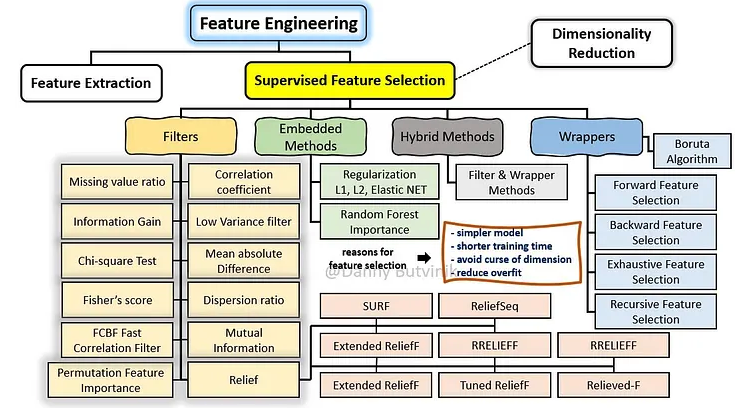
\includegraphics[scale=0.3]{cheat_sheet.png}
            \end{center}
        \end{figure}
    \end{frame}


    \section{MRMR Explained}
    \begin{frame}
        \frametitle{MRMR}
        MRMR works iteratively. At each iteration, it identifies the best feature (according to a
        rule) and adds it to the basket of selected features. Once a feature goes into the bucket,
        it cannot ever come out.
        \pause

        In each iteration $i$ a score is computed for each feature $f$ according to formula:
        \[
            score_i (f) = \frac{relevance(f|target)}{redundancy(f|\text{features selected until } (
            i-1))} \quad ,
        \]
        where we have to specify the relevancy and redundancy functions.

    \end{frame}

    \begin{frame}
        \frametitle{Feature importance}
        There are couple of variants to calculate the feature importance from the original UBER
        paper. For discrete features:
        \begin{itemize}
            \item Mutual Information Difference (MID):
            \[
                f^{MID}(X_i) = I(Y, X_i) - \frac{1}{|S|} \sum_{X_s \in S} I(X_s, X_i)]
            \]
            \pause
            \item Mutual Information Quotient (MIQ):
            \[
                f^{MID}(X_i) = I(Y, X_i) / \left( \frac{1}{|S|} \sum_{X_s \in S} I(X_s, X_i)] \right)
            \]
        \end{itemize}
    \end{frame}

    \begin{frame}
        \frametitle{Feature importance}
        For continues features:
        \begin{itemize}
            \item F-test Correlation Difference (FCD):
            \[
                f^{MID}(X_i) = F(Y, X_i) - \frac{1}{|S|} \sum_{X_s \in S} \rho (X_s, X_i)]
            \]
            \pause
            \item F-test Correlation Quotient (FCQ):
            \[
                f^{MID}(X_i) = F(Y, X_i) / \left( \frac{1}{|S|} \sum_{X_s \in S} \rho (X_s, X_i)] \right)
            \]
        \end{itemize}
        where $\rho$ is Pearson correlation.
    \end{frame}

    \begin{frame}
        \frametitle{Feature importance}
        Another extensions:
        \begin{itemize}
            \item RDC algorithm for redundancy function (The randomized dependence coefficient)
            \pause
            \item Model-based Feature importance for relevance:
                \begin{itemize}
                    \item Random Forest Correlation Quotient
                    \item Random Forest RDC Quotient
                    \item Pure Random Forest
                \end{itemize}
        \end{itemize}
        \pause
        From benchmarks, RF variances are good if down-stream model is Random Forest. FCQ is
        pretty close and works on more models.
    \end{frame}

    \begin{frame}
        \frametitle{Example}
        \begin{figure}
            \begin{center}
                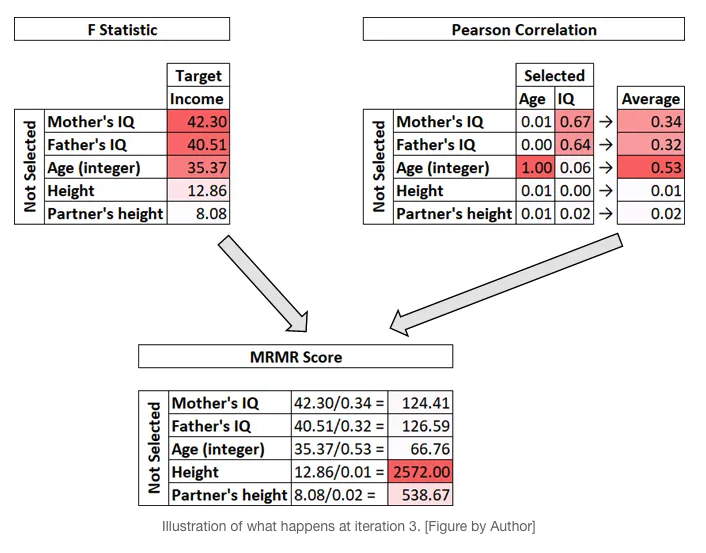
\includegraphics[scale=0.3]{fs_example.png}
            \end{center}
        \end{figure}
    \end{frame}

    \section{End of Story}
    \begin{frame}
        \frametitle{The End}
        Thank you for your attention and patience.
    \end{frame}


\end{document}
